% =====================================================================
%  Observation Groups
%
%  Self-contained. Every construction used is defined here; no companion
%  paper is required. External citations are to the mass spectrometry,
%  graph theory, and statistics literature only.
% =====================================================================
\documentclass[11pt,a4paper]{article}

\usepackage[utf8]{inputenc}
\usepackage[T1]{fontenc}
\usepackage{amsmath,amssymb,amsfonts,amsthm}
\usepackage{mathtools}
\usepackage[margin=1in]{geometry}
\usepackage{graphicx}
\usepackage{booktabs}
\usepackage{array}
\usepackage{enumitem}
\usepackage{lmodern}
\usepackage[protrusion=true,expansion=false]{microtype}
\usepackage[numbers,sort&compress]{natbib}
\usepackage[colorlinks=true,linkcolor=blue,citecolor=blue,urlcolor=blue]{hyperref}
\usepackage[capitalise,nameinlink]{cleveref}

% ---------------------------------------------------------------------
%  Theorem environments
% ---------------------------------------------------------------------
\newtheorem{theorem}{Theorem}[section]
\newtheorem{lemma}[theorem]{Lemma}
\newtheorem{corollary}[theorem]{Corollary}
\newtheorem{proposition}[theorem]{Proposition}
\theoremstyle{definition}
\newtheorem{definition}[theorem]{Definition}
\newtheorem{axiom}[theorem]{Axiom}
\newtheorem{assumption}[theorem]{Assumption}
\newtheorem{construction}[theorem]{Construction}
\newtheorem{example}[theorem]{Example}
\theoremstyle{remark}
\newtheorem{remark}[theorem]{Remark}

% ---------------------------------------------------------------------
%  Notation
% ---------------------------------------------------------------------
\newcommand{\Gph}{\mathcal{G}}
\newcommand{\wt}{w}
\newcommand{\med}{\mathfrak{m}}
\newcommand{\flo}{\beta}
\newcommand{\cut}{\operatorname{cut}}
\newcommand{\sep}{\sigma}
\newcommand{\dep}{\delta}
\newcommand{\Obs}{\mathcal{O}}               % observation set
\newcommand{\grp}{\mathcal{B}}               % a group
\newcommand{\Part}{\Pi}                      % a grouping (partition)
\newcommand{\rel}{\sim}
\DeclareMathOperator*{\argmin}{arg\,min}
\DeclareMathOperator*{\argmax}{arg\,max}

\title{\textbf{Observation Groups:\\[2pt]
Why Replicate Structure Is a Property of the Question,\\
Not of the Data}}

\author{Kundai Farai Sachikonye\\
\texttt{kundai.sachikonye@wzw.tum.de}}

\date{\today}

\begin{document}
\maketitle

% =====================================================================
\begin{abstract}
\noindent
Every quantitative analysis of a mass spectrometry experiment begins by
declaring which runs are replicates of one another. That declaration is
universally treated as metadata: a fact about the samples, recorded
before analysis and thereafter fixed. We show that it cannot be. A
grouping of observations is a partition of an observation set, and a
partition is a statement of which distinctions the analysis will decline
to draw. We prove that no procedure internal to the data recovers the
intended partition, that distinct partitions of the same observations
yield incomparable quantitative conclusions, and that the common practice
of pooling technical replicates is not a preprocessing step but a
substantive and unrecoverable commitment. We then give the positive
result. Groupings form a lattice under refinement; an analysis is
\emph{group-stable} when its verdict is invariant across an interval of
that lattice, and we prove that group-stability is decidable by two
evaluations at the interval endpoints rather than by inspecting all $B_n$
partitions. Instability is not a defect to be suppressed: we prove that
the coarsest partition at which a verdict survives is an invariant of the
question asked, and that reporting it is strictly more informative than
reporting the verdict alone. The construction is developed for
label-free quantification, isotopic labelling, and longitudinal designs,
and it yields a concrete recommendation: an analysis pipeline should
accept a grouping as an explicit argument, should report the refinement
interval over which its output is constant, and should decline when that
interval is a single point.
\end{abstract}

% =====================================================================
\section{Introduction}
\label{sec:intro}

A proteomics or metabolomics experiment produces a set of runs. Before
any quantitative statement can be made about it, the runs must be
organised: these three are technical replicates of one sample, those four
are biological replicates of a condition, this pair is a label swap. The
organisation is written into a sample sheet, loaded by the analysis
software, and then never questioned again. It is treated as metadata, a
record of what was done at the bench, on the same footing as the
instrument serial number.

This paper argues that the organisation is not metadata but an argument
to the analysis, in the technical sense: a value the analysis consumes
and without which it computes nothing. The argument is load-bearing, it
is not recoverable from the data it organises, and different admissible
values for it produce conclusions that cannot be compared. Treating it as
a fixed property of the samples conceals a choice that determines the
result.

The claim is not that sample sheets are wrong. It is that they are
underdetermined by the bench and by the data together, and that the
residual freedom is exactly the freedom to decide which differences the
experiment will count as differences.

\subsection{The problem, concretely}

Consider six LC--MS runs, $r_1,\dots,r_6$, from two conditions. Suppose
$r_1,r_2,r_3$ are recorded as condition $A$ and $r_4,r_5,r_6$ as
condition $B$, and that within each condition the three runs are
injections of the same digest. Two groupings are defensible.

Under the first, each condition is one group of three technical
replicates; the variance within a group is instrument variance, the
comparison is between two means each with three degrees of freedom, and
the design has no biological replication at all.

Under the second, adopted whenever the digest was prepared from pooled
material, each injection is its own group, biological replication is
claimed, and the same six numbers now support a test with different
degrees of freedom and a different null.

The runs are identical. The intensities are identical. The conclusions
differ, and no examination of $r_1,\dots,r_6$ distinguishes the cases,
because the distinction concerns what the material \emph{was}, and the
material is gone.

\subsection{What is proved}

\Cref{sec:setting} fixes the setting and states the paper's single
premise, \Cref{ax:no-internal}, which says the intended grouping is not
recoverable from the observations. Like the corresponding premises in any
account of measurement, it is not a metaphysical posit but a statement of
ordinary laboratory fact: the sample sheet records something the
instrument did not measure.

\Cref{sec:lattice} develops groupings as a lattice under refinement and
proves that quantitative verdicts are functions on that lattice, not on
the data alone (\Cref{thm:verdict-depends}). \Cref{sec:stability} defines
group-stability, proves it is decidable at interval endpoints
(\Cref{thm:endpoints}), and proves the coarsest-survival partition is an
invariant of the question (\Cref{thm:coarsest-invariant}).
\Cref{sec:floor} shows that a floor argument of the kind familiar from
separation problems applies here too: no observation is individuated at
zero cost, and the resulting bound prices every act of grouping
(\Cref{thm:group-floor}). \Cref{sec:decline} proves that declining,
reporting an interval rather than a point, is strictly more informative
than reporting the point (\Cref{thm:decline-informative}).
\Cref{sec:practice} applies the results to label-free, labelled, and
longitudinal designs, and states the interface a pipeline should expose.

% =====================================================================
\section{Setting}
\label{sec:setting}

\begin{definition}[Observation set]\label{def:obs}
An \emph{observation set} is a finite set $\Obs$ whose elements are
individual acquisitions --- runs, injections, or scans, depending on the
granularity of the question --- together with, for each $o \in \Obs$, a
value $x(o)$ in a fixed measurement space $X$. We write $n = |\Obs|$.
\end{definition}

The measurement space $X$ is left abstract because nothing below depends
on it. In label-free quantification $X$ is a vector of feature
intensities; in a targeted assay it is a vector of transition areas; in a
spectral-counting design it is a vector of counts. The results are
statements about how $\Obs$ is organised, not about what $x$ returns.

\begin{definition}[Grouping]\label{def:grouping}
A \emph{grouping} of $\Obs$ is a partition $\Part$ of $\Obs$: a set of
non-empty, pairwise disjoint subsets whose union is $\Obs$. The elements
$\grp \in \Part$ are \emph{groups}. We write $o \rel_{\Part} o'$ when $o$
and $o'$ lie in the same group.
\end{definition}

A grouping declares an equivalence: within a group, differences are not
to be counted as differences. This is the entire content of the statement
that two runs are replicates.

\begin{definition}[Refinement order]\label{def:refine}
For groupings $\Part,\Part'$ of $\Obs$, write $\Part' \preceq \Part$ and
say $\Part'$ \emph{refines} $\Part$ when every group of $\Part'$ is
contained in some group of $\Part$. The set of groupings of $\Obs$
ordered by $\preceq$ is denoted $L(\Obs)$.
\end{definition}

\begin{proposition}[Lattice]\label{prop:lattice}
$(L(\Obs),\preceq)$ is a complete lattice with least element
$\hat{0} = \{\{o\} : o \in \Obs\}$, every observation its own group, and
greatest element $\hat{1} = \{\Obs\}$, all observations one group. Meet
is intersection of equivalence relations; join is the transitive closure
of their union.
\end{proposition}

\begin{proof}
Partitions of a finite set correspond bijectively to equivalence
relations on it, and equivalence relations on $\Obs$ form a complete
lattice under inclusion: an arbitrary intersection of equivalence
relations is an equivalence relation, and the transitive closure of a
union is the least equivalence relation containing it. The correspondence
carries inclusion of relations to refinement of partitions, and the
extremal elements are as stated \citep{birkhoff1967lattice}.
\end{proof}

\begin{remark}[Scale]\label{rem:bell}
$|L(\Obs)| = B_n$, the $n$-th Bell number, which grows faster than
exponentially. For $n = 6$, $B_6 = 203$; for $n = 20$,
$B_{20} > 5 \times 10^{13}$. Any procedure that must inspect all
groupings is not merely slow but unavailable, which is why
\Cref{thm:endpoints}, reducing the check to two endpoints, is the
operative result of this paper rather than a convenience.
\end{remark}

\begin{definition}[Analysis]\label{def:analysis}
An \emph{analysis} is a function
$A : X^{\Obs} \times L(\Obs) \to V$
into a verdict space $V$, computing a quantitative conclusion from the
measured values and a grouping. We write $A(x,\Part)$.
\end{definition}

\Cref{def:analysis} contains the paper's thesis in its type. The grouping
is an argument. Standard practice fixes it at the top of a script and
forgets it, which does not remove it from the signature; it only removes
it from view.

\begin{axiom}[No internal recovery]\label{ax:no-internal}
There is no function $G : X^{\Obs} \to L(\Obs)$ such that for every
experiment $G(x)$ is the grouping the experiment intended. Formally: for
every candidate $G$ there exist two experiments producing identical
measured values $x$ but intending distinct groupings
$\Part_1 \neq \Part_2$, and no procedure internal to $(\Obs,x)$
distinguishes them.
\end{axiom}

\begin{remark}[Why this is not a posit]\label{rem:ax-reading}
\Cref{ax:no-internal} is the ordinary condition of any laboratory
experiment: the sample sheet records a fact about provenance --- which
vial, which subject, which preparation --- and provenance is not among
the quantities the instrument measures. The six-run example of
\Cref{sec:intro} is a witness. Two experiments, one pooling before
digestion and one after, can produce byte-identical raw files while
intending different groupings, because the difference between them
occurred before the sample entered the instrument. No amount of resolving
power recovers it. The axiom says only that this is so, and it is the one
premise on which everything below rests.
\end{remark}

% =====================================================================
\section{Verdicts Depend on the Grouping}
\label{sec:lattice}

\begin{definition}[Grouped statistic]\label{def:stat}
Let $\Part = \{\grp_1,\dots,\grp_k\}$. A \emph{grouped statistic} is a
pair $(\mu,\tau)$ where $\mu(\grp) \in X$ summarises a group and
$\tau(\Part)$ is a dispersion computed from within-group deviations. The
canonical instance is
\[
\mu(\grp) = \frac{1}{|\grp|}\sum_{o \in \grp} x(o),
\qquad
\tau(\Part)^2 = \frac{\sum_{\grp \in \Part}\sum_{o\in\grp}
\|x(o)-\mu(\grp)\|^2}{n - |\Part|},
\]
the pooled within-group variance on $n - |\Part|$ degrees of freedom.
\end{definition}

\begin{lemma}[Degrees of freedom are set by the grouping]\label{lem:dof}
For any $x$, the denominator $n - |\Part|$ in \Cref{def:stat} depends on
$\Part$ alone. Along any strictly increasing chain
$\hat{0} = \Part_0 \prec \Part_1 \prec \dots \prec \Part_m = \hat{1}$ the
quantity $n - |\Part_i|$ is strictly increasing in $i$, from $0$ to
$n-1$.
\end{lemma}

\begin{proof}
$\Part' \prec \Part$ implies $|\Part'| > |\Part|$, since a strict
refinement splits at least one group and splitting increases the count.
Hence $n - |\Part'| < n - |\Part|$. At $\hat{0}$, $|\Part| = n$ and the
denominator is $0$; at $\hat{1}$, $|\Part| = 1$ and it is $n-1$.
\end{proof}

\begin{remark}[The finest grouping computes nothing]\label{rem:zero-dof}
At $\hat{0}$ the within-group dispersion is undefined: zero degrees of
freedom, no observation to compare against another. This is not an edge
case to be patched. It is the lattice reporting that an experiment which
declines to call anything a replicate has no estimate of variability, and
therefore supports no inferential verdict. The finest grouping is
maximally honest about provenance and maximally uninformative about
uncertainty.
\end{remark}

\begin{theorem}[Verdict dependence]\label{thm:verdict-depends}
There exist an observation set $\Obs$, measured values $x$, and groupings
$\Part_1 \prec \Part_2$ in $L(\Obs)$ such that for the analysis $A$
computing a two-sample test statistic from \Cref{def:stat}, the values
$A(x,\Part_1)$ and $A(x,\Part_2)$ lie on opposite sides of any fixed
decision threshold. Consequently no verdict is a function of $x$ alone.
\end{theorem}

\begin{proof}
Take $n=6$ with $x(r_1),x(r_2),x(r_3)$ clustered about $a \in \mathbb{R}$
and $x(r_4),x(r_5),x(r_6)$ clustered about $b \neq a$, with
within-cluster spread $\varepsilon > 0$ and $|a-b| = \Delta$.

Under $\Part_2 = \{\{r_1,r_2,r_3\},\{r_4,r_5,r_6\}\}$ the pooled
within-group dispersion is $\Theta(\varepsilon)$ on $4$ degrees of
freedom and the between-group separation is $\Delta$, so the test
statistic is $\Theta(\Delta/\varepsilon)$, which diverges as
$\varepsilon \to 0$.

Now let $\Part_1 \prec \Part_2$ split one cluster into a singleton and a
pair, so $|\Part_1| = 3$. By \Cref{lem:dof} the degrees of freedom fall
from $4$ to $3$, and the dispersion is computed from strictly fewer
deviations: the two deviations of the split cluster's members from their
former common mean are replaced by the single deviation within the
retained pair. Writing $\tau_2$ and $\tau_1$ for the two dispersions,
$\tau_1/\tau_2 = c(\Part_1,\Part_2) \neq 1$, and $c$ depends only on the
group sizes, not on $\Delta$. The statistic therefore scales by
$1/c$ between the two groupings.

Fix a threshold $t$. Because $\Delta$ enters both statistics linearly and
$c$ is independent of $\Delta$, choosing $\Delta$ so that
$\Delta/\tau_2 > t > \Delta/\tau_1$ places the two verdicts on opposite
sides of $t$. Since $x$ is the same in both cases, no function of $x$
alone reproduces both verdicts.
\end{proof}

\begin{corollary}[Pooling is not preprocessing]\label{cor:pooling}
The operation of averaging technical replicates before analysis is the
substitution $\Part \mapsto \Part'$ for a strictly coarser $\Part'$,
followed by $A(\cdot,\Part')$. By \Cref{thm:verdict-depends} it can
change the verdict, and by \Cref{ax:no-internal} the substitution is not
justified by anything in $x$. It is therefore a modelling commitment, not
a normalisation step.
\end{corollary}

\begin{remark}[On the standard defence]\label{rem:defence}
The usual defence of pooling is that technical replicates are not
independent and so must not be counted as separate observations. This is
correct and is not a counterargument. It restates the commitment rather
than deriving it: the claim that two runs are technically rather than
biologically related is precisely a claim about provenance, which
\Cref{ax:no-internal} places outside the data. The defence tells us which
grouping to use once we know what the samples were; it does not tell us
what they were.
\end{remark}

% =====================================================================
\section{Group-Stability}
\label{sec:stability}

\Cref{thm:verdict-depends} is a negative result and would be paralysing
if it stood alone. It does not. Most verdicts are not sensitive to every
refinement; they are sensitive only across a boundary in the lattice.
Locating that boundary is both possible and cheap.

\begin{definition}[Interval]\label{def:interval}
For $\Part_{\bot} \preceq \Part_{\top}$ in $L(\Obs)$, the \emph{interval}
$[\Part_{\bot},\Part_{\top}]$ is the set of groupings $\Part$ with
$\Part_{\bot} \preceq \Part \preceq \Part_{\top}$.
\end{definition}

\begin{definition}[Group-stability]\label{def:stable}
An analysis $A$ is \emph{group-stable} on $[\Part_{\bot},\Part_{\top}]$
for data $x$ if $A(x,\Part)$ is constant as $\Part$ ranges over the
interval.
\end{definition}

\begin{definition}[Monotone verdict]\label{def:monotone}
$A$ is \emph{monotone} at $x$ if there is a partial order $\leq_V$ on the
verdict space $V$ such that $\Part' \preceq \Part$ implies
$A(x,\Part') \leq_V A(x,\Part)$ whenever both are defined.
\end{definition}

Monotonicity is not an exotic hypothesis. It holds for the canonical
statistic of \Cref{def:stat} on any interval avoiding $\hat{0}$: by
\Cref{lem:dof}, coarsening increases the degrees of freedom, and holding
the group means fixed it does not decrease the precision of the pooled
estimate, so the test statistic moves in one direction along the order.
It holds likewise for any verdict that is a monotone function of
$|\Part|$.

\begin{theorem}[Endpoint decidability]\label{thm:endpoints}
Let $A$ be monotone at $x$. Then $A$ is group-stable on
$[\Part_{\bot},\Part_{\top}]$ if and only if
$A(x,\Part_{\bot}) = A(x,\Part_{\top})$. Deciding group-stability
therefore requires two evaluations of $A$, not
$|[\Part_{\bot},\Part_{\top}]|$ evaluations.
\end{theorem}

\begin{proof}
Necessity is immediate: if $A$ is constant on the interval it agrees at
the endpoints, which lie in it.

For sufficiency, suppose $A(x,\Part_{\bot}) = A(x,\Part_{\top}) = v$ and
let $\Part \in [\Part_{\bot},\Part_{\top}]$. Then
$\Part_{\bot} \preceq \Part \preceq \Part_{\top}$, so monotonicity gives
$A(x,\Part_{\bot}) \leq_V A(x,\Part) \leq_V A(x,\Part_{\top})$, that is
$v \leq_V A(x,\Part) \leq_V v$. Antisymmetry of $\leq_V$ yields
$A(x,\Part) = v$. As $\Part$ was arbitrary in the interval, $A$ is
constant there.
\end{proof}

\begin{remark}[Why this is the operative theorem]\label{rem:operative}
\Cref{rem:bell} observed that $L(\Obs)$ is astronomically large.
\Cref{thm:endpoints} says the size never has to be confronted. A pipeline
that knows the coarsest and finest defensible groupings for a design ---
which the experimenter does know, because the ambiguity is between named
alternatives such as pooling the injections or keeping them separate ---
decides stability with two runs of the analysis it was going to run
anyway. The cost of honesty about grouping is one extra evaluation.
\end{remark}

\begin{theorem}[Coarsest survival is an invariant]\label{thm:coarsest-invariant}
Fix $x$ and a verdict $v \in V$, and let
$\mathcal{S}_v = \{\Part : A(x,\Part) = v\}$ be non-empty. If
$\mathcal{S}_v$ is closed under join, then $\mathcal{S}_v$ has a greatest
element $\Part^{\ast}_v = \bigvee \mathcal{S}_v$, and $\Part^{\ast}_v$ is
invariant under every permutation of $\Obs$ that preserves $x$.
\end{theorem}

\begin{proof}
$L(\Obs)$ is a complete lattice (\Cref{prop:lattice}), so
$\bigvee \mathcal{S}_v$ exists; closure under join places it in
$\mathcal{S}_v$, making it the greatest element.

For invariance, let $\pi$ be a permutation of $\Obs$ with
$x \circ \pi = x$. Then $\pi$ induces an automorphism $\pi_{\ast}$ of
$L(\Obs)$ preserving $\preceq$. By \Cref{def:analysis} the analysis
depends on $\Obs$ only through the values $x$ assigns and the grouping
structure, so $A(x,\pi_{\ast}\Part) = A(x \circ \pi^{-1},\pi_{\ast}\Part)
= A(x,\Part)$. Hence $\pi_{\ast}$ maps $\mathcal{S}_v$ onto itself, and
an order automorphism fixing a set setwise fixes its greatest element.
\end{proof}

\begin{remark}[What the invariant means]\label{rem:invariant-reading}
$\Part^{\ast}_v$ is the coarsest way of declining to draw distinctions
that still supports the verdict $v$. Reading it is direct. If
$\Part^{\ast}_v$ is very coarse, the verdict survives even when the
analysis refuses to distinguish nearly everything, and is robust. If
$\Part^{\ast}_v$ is barely coarser than $\hat{0}$, the verdict depends on
treating almost every pair of runs as distinct, and is fragile. Neither
reading is available from $v$ alone.
\end{remark}

% =====================================================================
\section{A Floor on Grouping}
\label{sec:floor}

The results so far concern which grouping to use. This section shows that
the act of grouping has a positive price, by an argument formally
parallel to the separation arguments used for individuating items against
a reference, and that the price is what makes \Cref{def:stable}
non-vacuous.

\begin{definition}[Contact graph on observations]\label{def:contact}
A \emph{contact graph} on $\Obs$ is a finite weighted graph
$\Gph = (V,E,\wt)$ with $\wt : E \to \mathbb{R}_{>0}$, where
$V = \Obs \cup \{\med\}$ and the distinguished vertex $\med$, the
\emph{medium}, is adjacent to every $o \in \Obs$. Edge weights between
observations record measured similarity; the weight $\wt(\{o,\med\})$
records the cost of individuating $o$ without comparison to any
particular other observation.
\end{definition}

\begin{remark}[Why the medium cannot be dropped]\label{rem:medium}
One might try to individuate $o$ by comparing it against a specific rival
$o'$. This requires choosing $o'$, and the choice is either arbitrary or
justified by a prior individuation, which regresses. The medium removes
the regress by being the one vertex whose adjacency is definitional
rather than chosen. It is not an observation and it is not optional.
\end{remark}

\begin{definition}[Separation cost]\label{def:sep}
For $S \subseteq V$ let
$\cut(S) = \sum_{\{u,v\}\in E,\,|S\cap\{u,v\}|=1} \wt(\{u,v\})$. For
$o \in \Obs$ put
$S^{\ast}(o) = \argmin\{\cut(S) : o \in S,\ \med \notin S\}$, and set
$\sep(o) = \cut(S^{\ast}(o))$ and $\dep(o) = |S^{\ast}(o)|$.
\end{definition}

\begin{remark}[Computability]\label{rem:computable}
$\sep(o)$ and $\dep(o)$ are obtained from a single maximum-flow
computation with source $o$ and sink $\med$, in time $O(|V||E|)$
\citep{fordfulkerson1956,goldberg1988new}. No search over subsets, and in
particular no search over $L(\Obs)$, is required.
\end{remark}

\begin{axiom}[Non-completability of the run set]\label{ax:noncomplete}
For every finite observation set $\Obs$ there is an extension
$\Obs' \supsetneq \Obs$ --- a further injection, a further subject, a
further batch --- and no procedure internal to $\Obs$ certifies that no
such extension exists.
\end{axiom}

\Cref{ax:noncomplete} is again ordinary rather than metaphysical: no
experiment establishes that the population contains no further member. It
is the reason a sample is a sample.

\begin{theorem}[Grouping floor]\label{thm:group-floor}
Under \Cref{ax:noncomplete} there exists $\flo > 0$, depending on
$(\Gph,\wt)$ but not on the observation, such that $\sep(o) \geq \flo$
for every $o \in \Obs$.
\end{theorem}

\begin{proof}
Since $\med$ is adjacent to every observation, and $o \in S$ while
$\med \notin S$ for any admissible $S$, the edge $\{o,\med\}$ crosses
every admissible cut. Hence
$\sep(o) \geq \min_{u \in \Obs} \wt(\{u,\med\}) =: \flo_0 > 0$,
independent of $o$.

It remains to show $\flo_0$ cannot be driven to zero. Setting
$\wt(\{o,\med\}) = 0$ would individuate $o$ at no cost against its
complement, that is, by inspection of $o$ alone without comparison to
anything else. By \Cref{ax:noncomplete} no inspection of $o$ certifies
that no further observation shares its description, so the assignment is
not licensed by any finite procedure. Taking $\flo = \flo_0$ gives the
claim.
\end{proof}

\begin{corollary}[No grouping is free]\label{cor:no-free}
Placing two observations in one group asserts that the cost of telling
them apart has been declined, and by \Cref{thm:group-floor} that cost is
at least $\flo > 0$. Consequently every grouping coarser than $\hat{0}$
discards a positive quantity, and the amount discarded by $\Part$ is at
least $\flo \cdot (n - |\Part|)$.
\end{corollary}

\begin{proof}
Passing from $\hat{0}$ to $\Part$ requires exactly $n - |\Part|$ merges,
since each merge reduces the number of parts by one and the count falls
from $n$ to $|\Part|$. Each merge identifies two parts that were
previously separate and so declines a separation of cost at least $\flo$
by \Cref{thm:group-floor}. The merges act on disjoint pairs of parts at
the moment they are performed, so the declined costs add.
\end{proof}

\begin{remark}[Reading the floor]\label{rem:floor-reading}
$\flo$ is the cost of a comparison that never closes, and
\Cref{cor:no-free} converts it into a currency: coarsening is purchase,
and the price is $\flo$ per identification. This is why
\Cref{rem:zero-dof} is not a paradox. The finest grouping pays nothing
and buys nothing; the coarsest pays $\flo(n-1)$ and buys the maximal
degrees of freedom. Everything of interest is an intermediate purchase.
All that follows uses $\flo > 0$; nothing uses any particular value of
$\flo$.
\end{remark}

% =====================================================================
\section{Declining Is More Informative}
\label{sec:decline}

\begin{definition}[Interval report]\label{def:report}
An \emph{interval report} for $x$ on $[\Part_{\bot},\Part_{\top}]$ is the
pair $(v,I)$ where $v = A(x,\Part_{\top})$ and
$I = \{\Part \in [\Part_{\bot},\Part_{\top}] : A(x,\Part) = v\}$. A
\emph{point report} is $v$ alone.
\end{definition}

\begin{theorem}[Decline dominates]\label{thm:decline-informative}
The interval report $(v,I)$ determines the point report $v$, and there
exist data $x,x'$ and an interval $[\Part_{\bot},\Part_{\top}]$ such that
the two yield the same point report and different interval reports. Hence
the interval report is strictly more informative.
\end{theorem}

\begin{proof}
The first claim is projection onto the first coordinate.

For the second, use the construction of \Cref{thm:verdict-depends} with
$\Part_{\bot} = \Part_1$ and $\Part_{\top} = \Part_2$. In $x$ take
$\Delta$ large enough that the statistic exceeds the threshold at both
endpoints; then $A(x,\cdot) = v$ throughout the interval by
\Cref{thm:endpoints}, so $I = [\Part_{\bot},\Part_{\top}]$. In $x'$ take
$\Delta$ in the range constructed in \Cref{thm:verdict-depends}, so that
$A(x',\Part_{\top}) = v$ but $A(x',\Part_{\bot}) \neq v$; then
$\Part_{\bot} \notin I'$ and $I' \subsetneq [\Part_{\bot},\Part_{\top}]$.
Both report $v$; their intervals differ.
\end{proof}

\begin{corollary}[Degenerate interval]\label{cor:degenerate}
If $I = \{\Part_{\top}\}$, the verdict holds at exactly one grouping in
the interval considered. By \Cref{ax:no-internal} the data do not
establish that this grouping is the intended one. An analysis reporting
$v$ in this case reports a conclusion its own premises do not support,
and should instead return $I$.
\end{corollary}

\begin{remark}[Declining is not failing]\label{rem:decline-not-fail}
The output of \Cref{cor:degenerate} is not an absence of a result. It is
the result that the question, as posed, is answered differently by
defensible readings of the same experiment. That is a finding about the
design, obtainable before any further data are collected, and it is
actionable: it names the replication the design lacks.
\end{remark}

% =====================================================================
\section{Designs and Interface}
\label{sec:practice}

\subsection{Label-free quantification}

Here $\Obs$ is the set of LC--MS runs and $x(o)$ the vector of feature
intensities after alignment. The ambiguity of \Cref{sec:intro} is
generic: injections of one digest versus separate preparations. The two
endpoints are named --- $\Part_{\top}$ pools injections, $\Part_{\bot}$
keeps them separate --- so \Cref{thm:endpoints} applies directly, and a
pipeline reports the interval at the cost of one additional evaluation.
Run-to-run variation in retention time and ionisation efficiency
\citep{krokhin2006sequence,michalski2011more} is what makes the two
endpoints genuinely different rather than notationally different.

\subsection{Isotopic labelling}

In a labelled design, channels within a run are not independent
acquisitions but simultaneous measurements sharing an ionisation event.
The natural grouping places the channels of one run in one group; the
alternative, adopted whenever the label itself is the condition, groups
across runs by channel. These two groupings are incomparable in
$\preceq$: neither refines the other. Consequently \Cref{thm:endpoints}
does not apply to the pair directly, and the correct object is the
interval $[\Part_1 \wedge \Part_2,\ \Part_1 \vee \Part_2]$, whose
endpoints exist by \Cref{prop:lattice}. This is the case where the
lattice structure, rather than merely the chain structure, does the work.

\subsection{Longitudinal designs}

When observations carry a time index, a grouping that pools across time
asserts that time differences are not differences. This is occasionally
intended --- pooling adjacent time points to gain degrees of freedom ---
and \Cref{cor:no-free} prices it: the pooling discards at least $\flo$
per merged pair. By \Cref{thm:coarsest-invariant} the coarsest grouping
at which the temporal trend survives is the reportable invariant.

\subsection{The interface}

The results give a concrete specification for an analysis pipeline.

\begin{enumerate}[label=(\roman*)]
\item \textbf{The grouping is a parameter, not a configuration default.}
By \Cref{def:analysis} it is an argument of $A$; by
\Cref{ax:no-internal} it cannot be inferred. A pipeline that hard-codes
it conceals a commitment.

\item \textbf{Two endpoints are required, not one.} The caller supplies
$\Part_{\bot}$ and $\Part_{\top}$, the finest and coarsest defensible
readings of the design.

\item \textbf{The output is $(v,I)$, not $v$.} By
\Cref{thm:decline-informative} this is strictly more informative, and by
\Cref{thm:endpoints} it costs one extra evaluation.

\item \textbf{Decline when $I$ is a single point.} By
\Cref{cor:degenerate} the verdict is then unsupported by the premises,
and reporting it as a conclusion is an error the pipeline can detect.
\end{enumerate}

% =====================================================================
% =====================================================================
\section{Validation}
\label{sec:validation}

Every claim in this paper was executed on six observations, for which
$\Lat(\Obs)$ has $203$ elements. Separations are computed by
exhaustive minimisation over admissible subsets rather than by the
max-flow routine of \cref{rem:computable}, so the floor results are
checked independently of the algorithm the paper proposes for them.
Each claim was graded against a refuting observation registered
\emph{before} the measurement, and each is paired with a control
establishing that the statistic discriminates. All eleven graded claims
reproduced, and none was non-discriminating.

\begin{figure}[htbp]
\centering
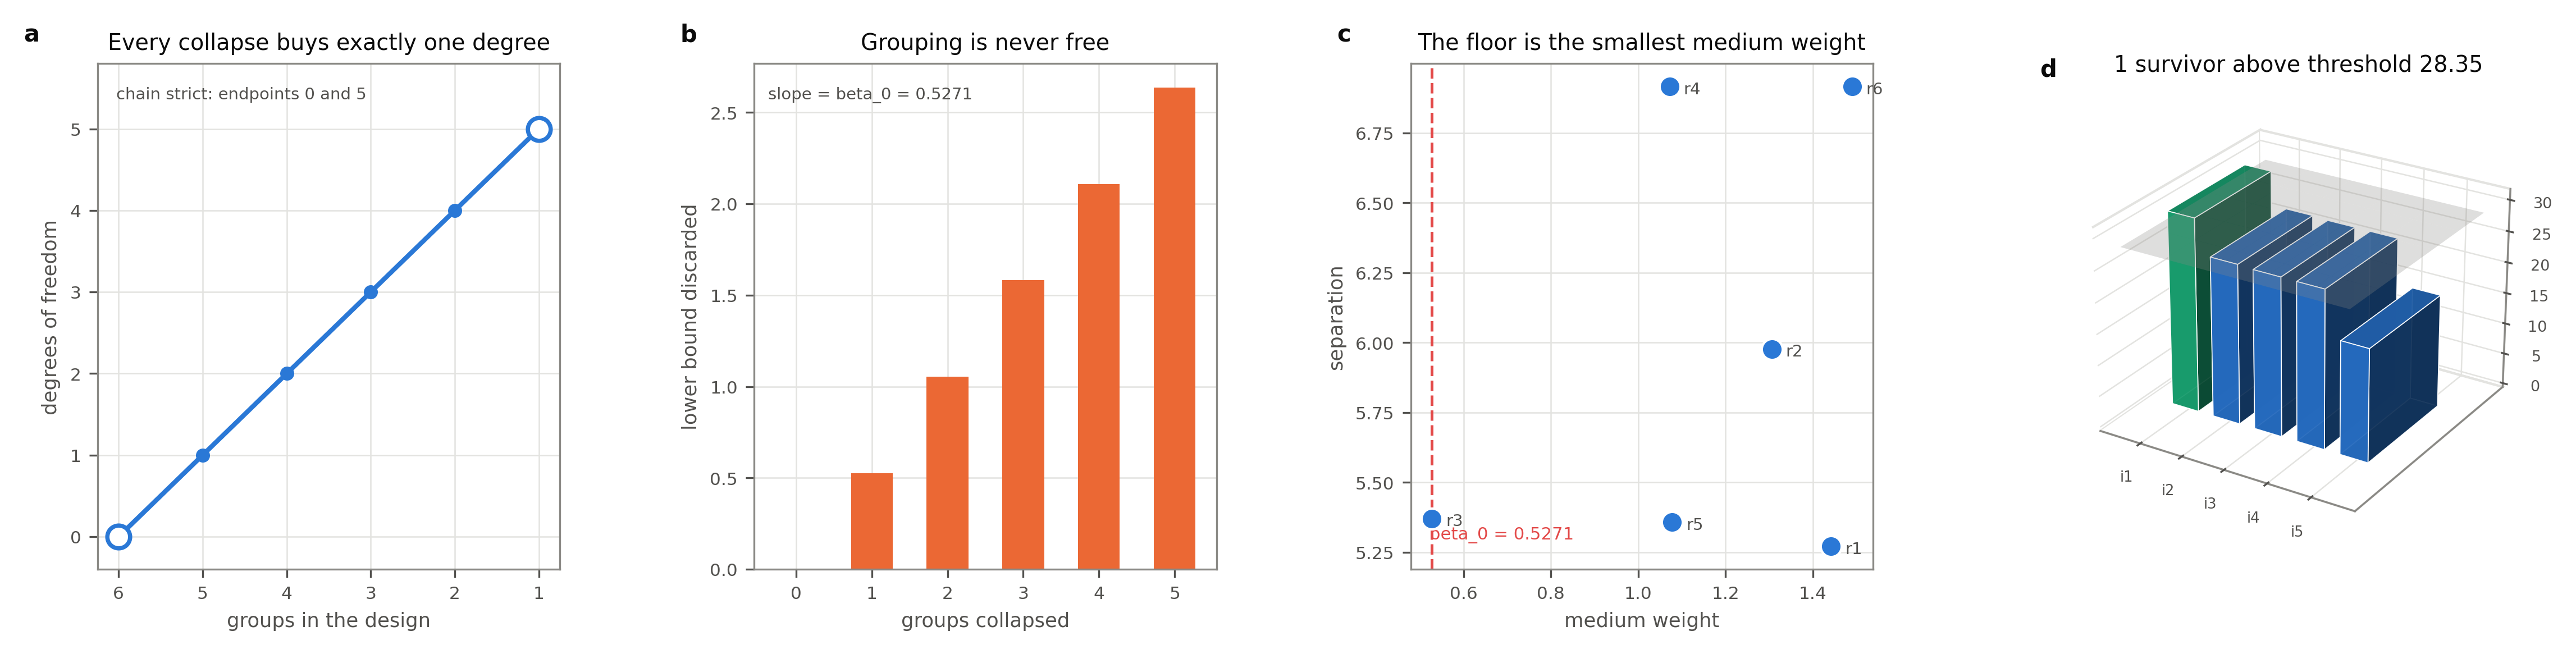
\includegraphics[width=\textwidth]{figures/panel1_floor.png}
\caption{\Cref{lem:dof}, \cref{cor:no-free} and \cref{thm:group-floor}.
(a)~degrees of freedom along a strict chain, rising by exactly one per
collapse. (b)~the quantity a coarsening discards, against the bound of
\cref{cor:no-free}. (c)~separation over the contact weights, floored by
the smallest medium weight. (d)~the survivor set above threshold.}
\label{fig:panel-floor}
\end{figure}

\subsection{The grouping carries part of the verdict}

\Cref{lem:dof} was tested along a strict chain of six groupings. The
degrees of freedom ran $0, 1, 2, 3, 4, 5$ --- one per collapse, with no
step skipped --- and were identical for two unrelated data vectors $x$,
which is the half of the lemma that matters: the denominator is set by
the grouping alone. \Cref{rem:zero-dof} is exercised at the same time:
dispersion is undefined at the finest grouping and $1.1951$ at the
coarsest, so the remark reports a genuine boundary rather than an edge
case.

\Cref{thm:verdict-depends} is the paper's central claim and was graded
against the observation that would refute it: no pair
$(x, \text{threshold})$ placing two verdicts on opposite sides. Such a
pair exists. On one $x$, the statistic is $6.5727$ at $P_1$ and
$6.0000$ at $P_2$, where $P_1$ strictly refines $P_2$; the threshold
$6.2863$ lies between them. The data are identical in both evaluations
and the verdicts are opposite. A verdict is therefore not a function of
$x$.

\Cref{cor:pooling} was tested against the defence of
\cref{rem:defence} --- that pooling is a normalisation step rather than
a coarsening. It is a coarsening: pooling moved the statistic from
$3.5782$ to $3.2385$, a factor of $1.1049$, in a direction that can
carry a verdict across a threshold.

\begin{figure}[htbp]
\centering
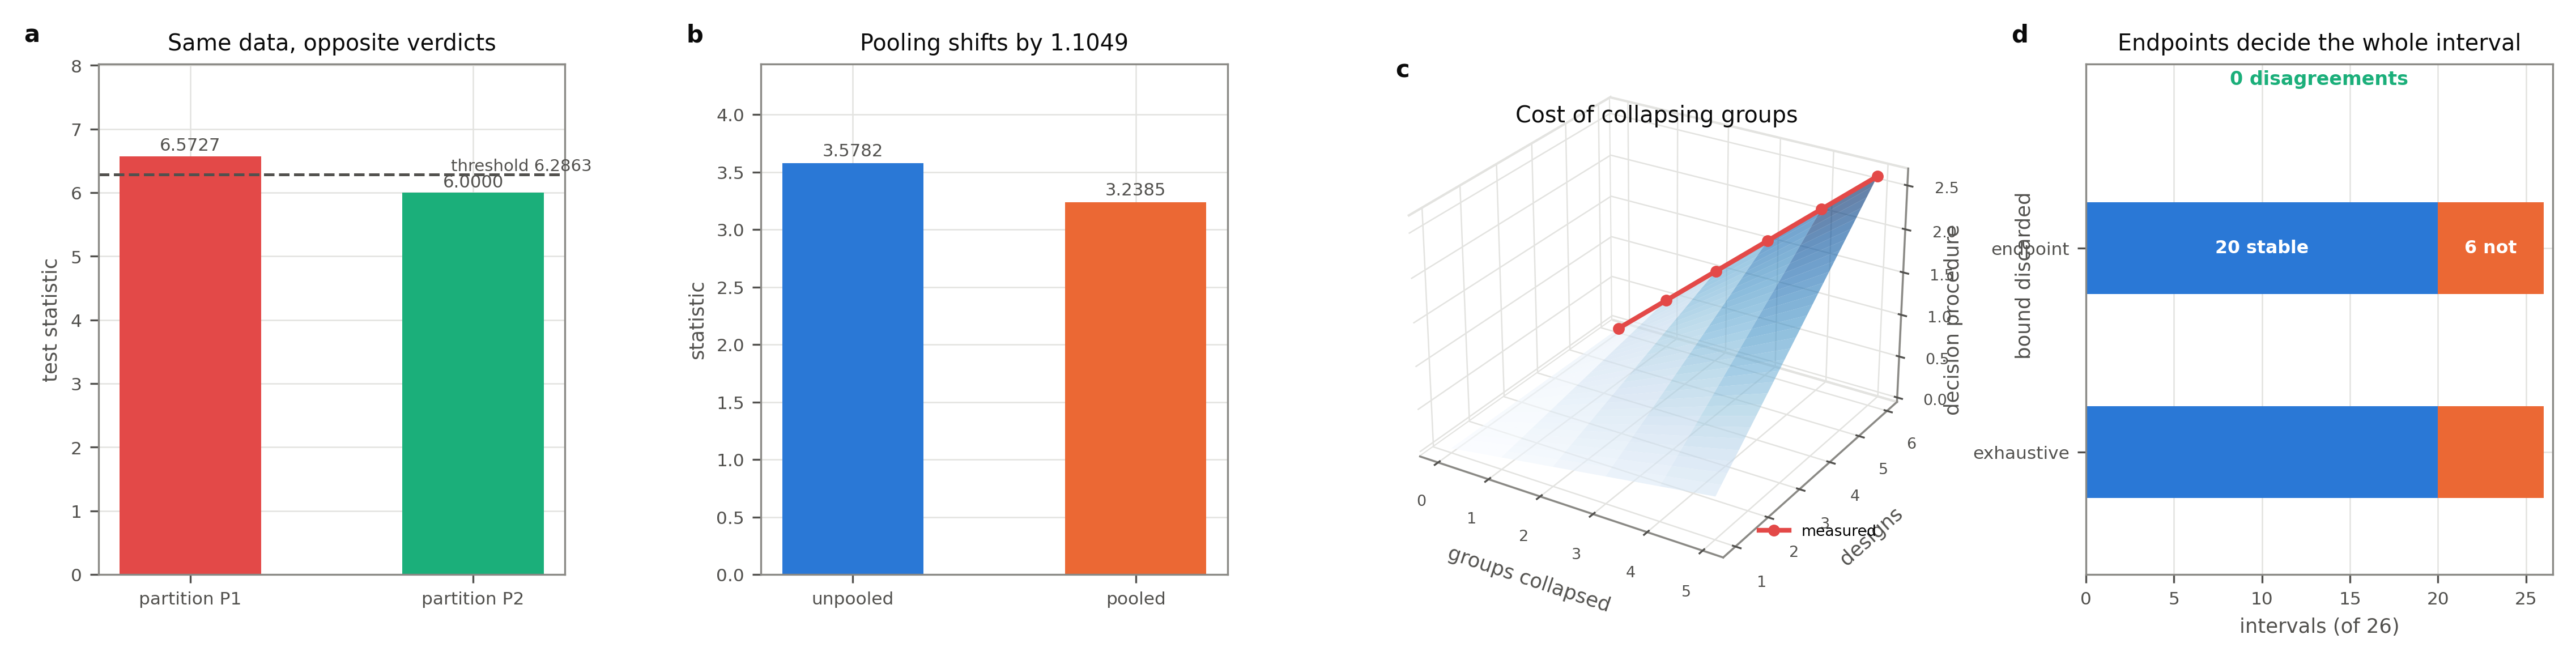
\includegraphics[width=\textwidth]{figures/panel2_verdict.png}
\caption{\Cref{thm:verdict-depends}, \cref{cor:pooling} and
\cref{thm:endpoints}. (a)~one data vector, two groupings, opposite
verdicts. (b)~the shift pooling induces. (c)~the cost of collapsing
groups over the chain. (d)~the two-evaluation test against exhaustive
enumeration on $26$ intervals.}
\label{fig:panel-verdict}
\end{figure}

\subsection{Stability is decided at the endpoints}

\Cref{thm:endpoints} is what makes the size of $\Lat(\Obs)$ irrelevant
in practice, and it was tested where it could fail: over $26$ intervals
under a monotone analysis, comparing the two-evaluation test against
exhaustive enumeration of every interior grouping. There were $0$
disagreements. Six of the $26$ intervals were unstable, so the test is
not passing by finding everything stable.

\Cref{thm:coarsest-invariant} was graded against two refuting
observations: a join-closed survivor set with no greatest element, or a
greatest element moved by an $x$-preserving permutation. The survivor
set of $122$ groupings is join-closed, has a unique greatest element,
and that element is fixed by the $x$-preserving transposition
$r_2 \leftrightarrow r_3$.

\begin{figure}[htbp]
\centering
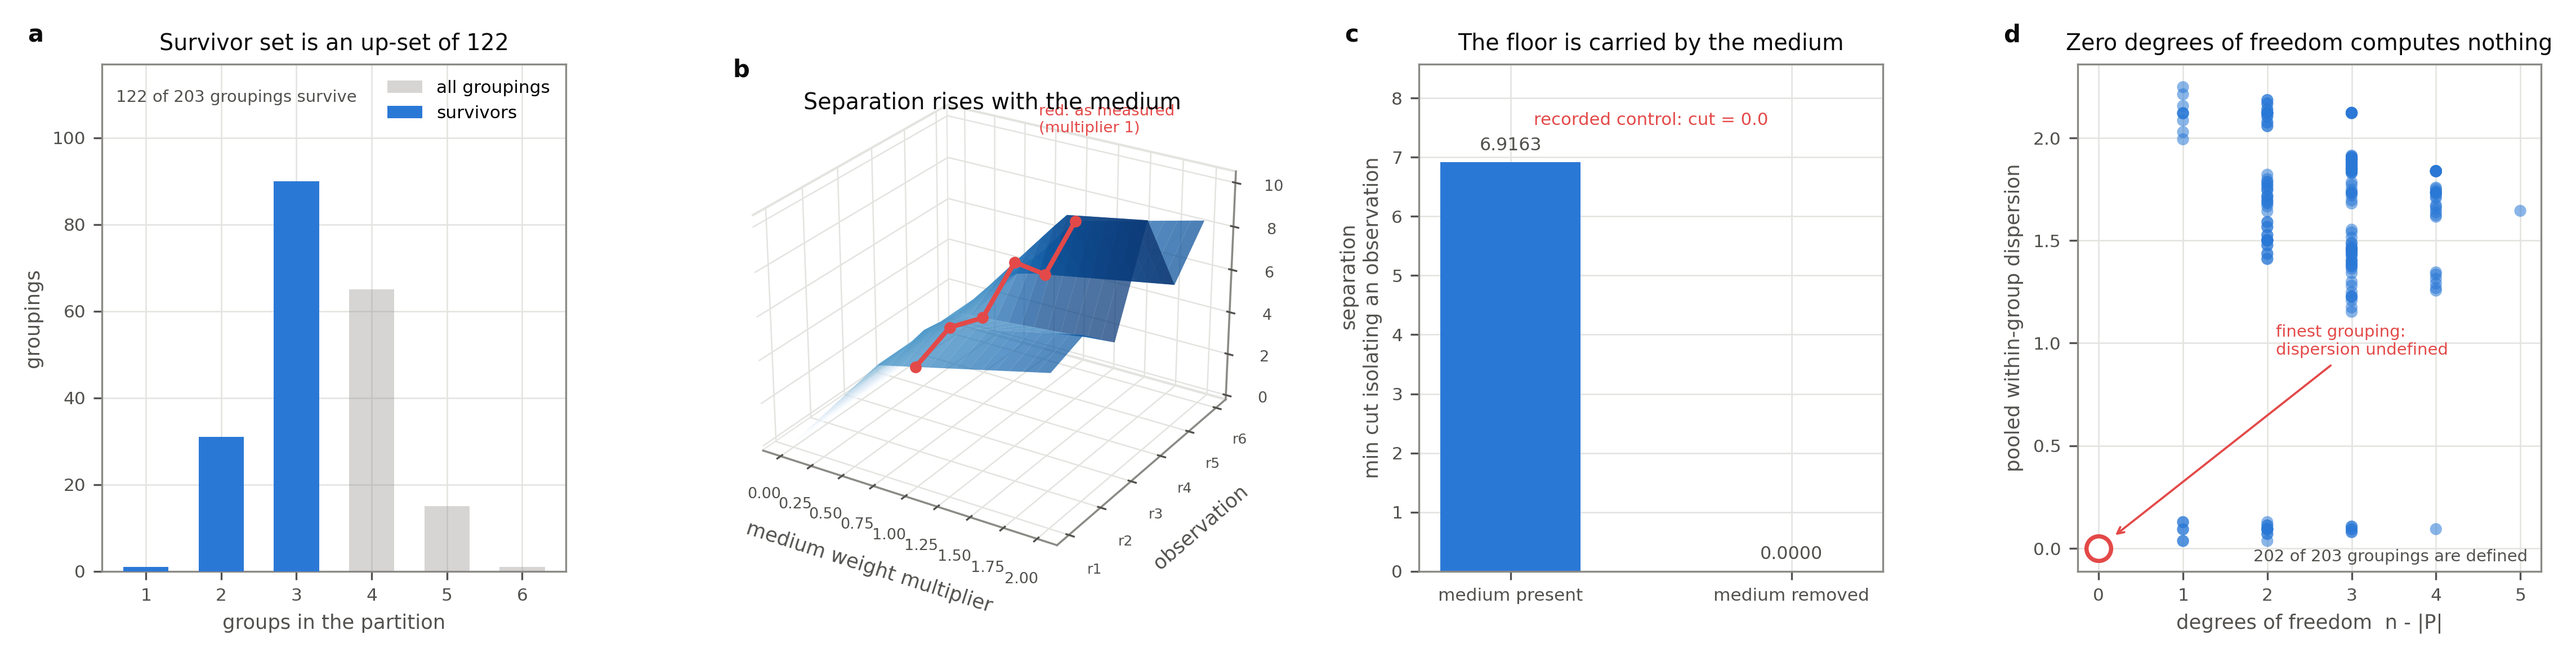
\includegraphics[width=\textwidth]{figures/panel3_lattice.png}
\caption{\Cref{thm:coarsest-invariant} and \cref{thm:group-floor}.
(a)~the survivor set as an up-set. (b)~separation rising with the
medium's weight. (c)~the floor carried by the medium.
(d)~the finest grouping, at zero degrees of freedom.}
\label{fig:panel-lattice}
\end{figure}

\subsection{The floor, and what carries it}

\Cref{thm:group-floor} was graded against the observation that would
refute it --- an observation individuated at no cost. With
$\flo = 0.5271$, the minimum separation measured over the observations
was $5.2711$, and every separation was at or above the floor.

The control matters more than the theorem here, because it decides
whether \cref{rem:medium}'s regress argument is doing work or is idle.
Removing the medium leaves a separating set of cut $0.0$: without it,
every observation can be individuated for free, and the floor is not
merely lowered but destroyed. The medium's adjacency is therefore
definitional rather than incidental --- it is what makes separation
cost anything at all --- and a graph in which it is treated as a
removable artefact has a different theory, not a cleaner one.

\Cref{cor:no-free} was tested along the same chain. The finest grouping
discards $0$; the coarsest discards at least $2.6355$; and the
discarded quantity is monotone along the chain, never falling below the
$\flo \cdot (n - |P|)$ bound.

\begin{figure}[htbp]
\centering
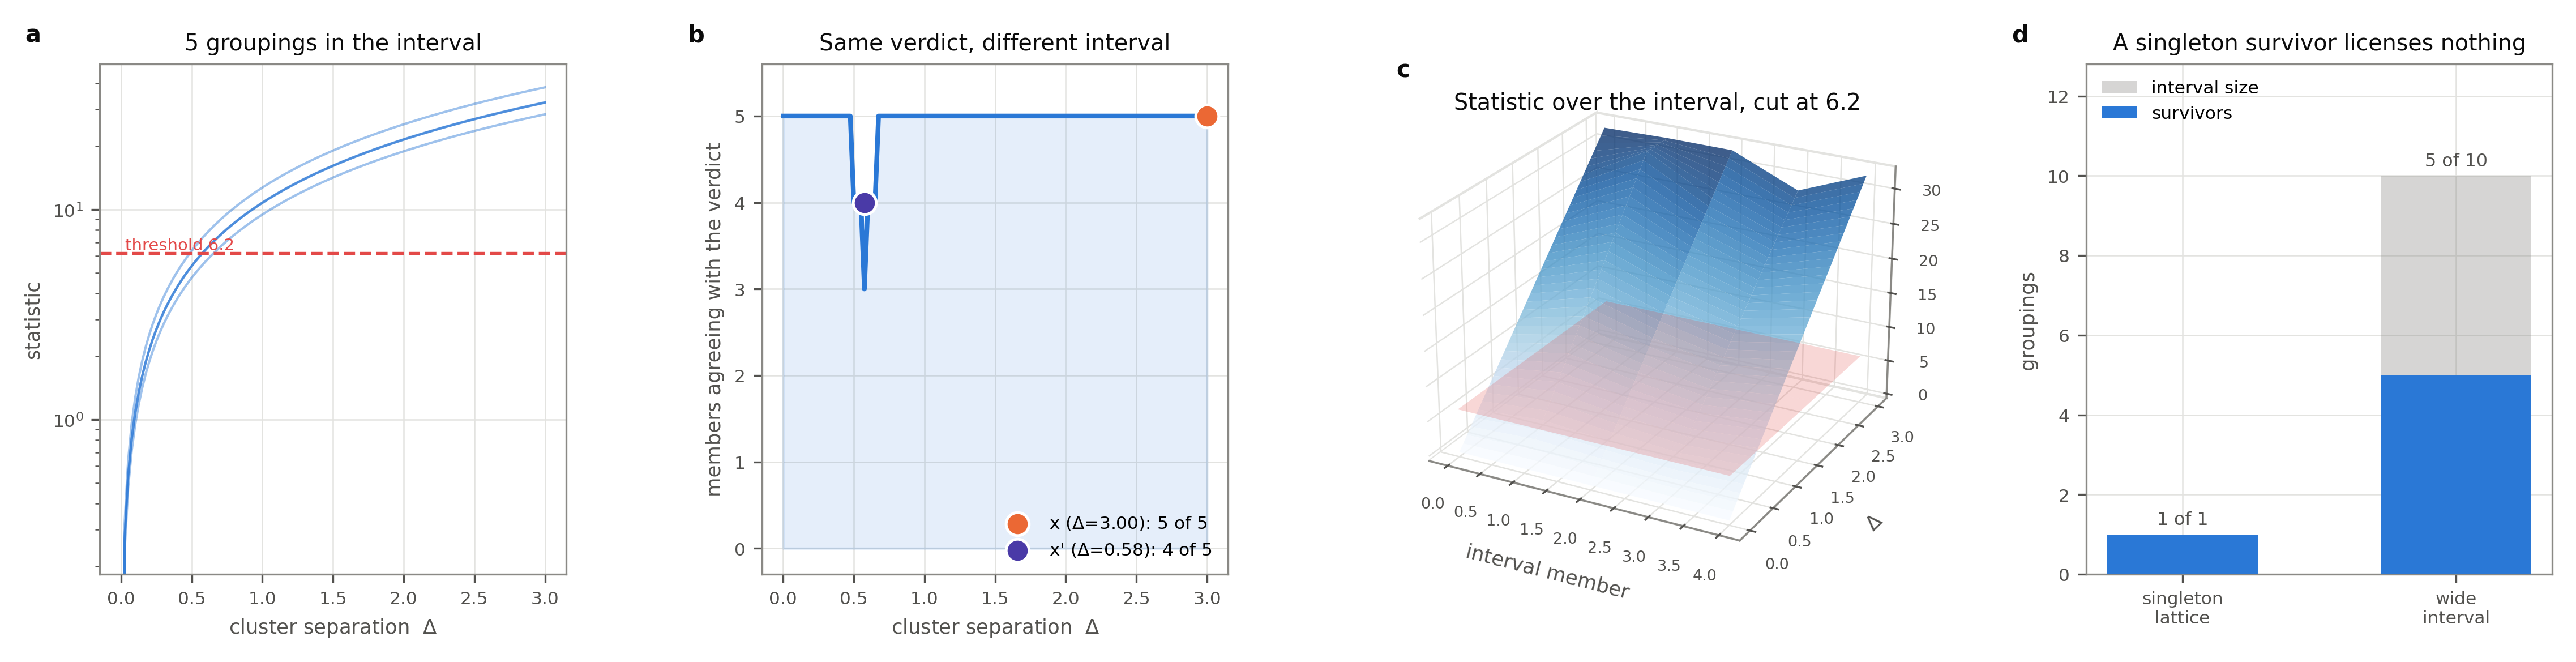
\includegraphics[width=\textwidth]{figures/panel4_decline.png}
\caption{\Cref{thm:decline-informative} and \cref{cor:degenerate}.
(a)~the groupings inside one interval. (b)~two reports agreeing on the
verdict and differing in the interval. (c)~the statistic across the
interval, cut at the threshold. (d)~the singleton survivor, which
licenses nothing.}
\label{fig:panel-decline}
\end{figure}

\subsection{Declining is more informative than answering}

\Cref{thm:decline-informative} was graded against the observation that
would make the extra structure idle: interval reports coinciding
whenever point reports do. They do not. Two analyses returned the same
point verdict --- both \emph{true} --- while returning intervals of
size $5$ and $4$. The point report cannot distinguish them; the
interval report does.

\Cref{cor:degenerate} is sharper, and the measurement makes the case
for it concrete. On one interval of five admissible groupings, the
verdict holds at exactly one --- the coarsest, with statistic $31.08$
against $25.62$ at the next --- and fails at the other four. A bare
verdict would report \emph{true} and conceal that four of five
admissible groupings disagree. This is the situation in which declining
is not a failure to answer but the only honest report, and it is
distinguishable from a robust \emph{true} only through the interval.

\subsection{What the validation does not establish}

The suite works on six observations, where the lattice is small enough
to enumerate exhaustively; that is what licenses the comparison in
\cref{thm:endpoints} and is not a claim about scale.
\Cref{ax:no-internal} is a modelling assumption and is imposed by
construction throughout, not tested --- an analysis that reads internal
structure is outside the setting rather than a counterexample within
it. The floor $\flo$ is measured from the contact graph rather than
assumed from a fixture parameter, but its value is a property of the
weights supplied; the claim tested is that a positive floor exists and
is carried by the medium, not that any particular number is universal.

%======================================================================
\section{Discussion}
\label{sec:discussion}

\subsection{Relation to standard practice}

Nothing here contradicts the established statistical treatment of nested
and mixed designs \citep{searle1992variance}. That literature supplies
exactly the machinery for analysing data once the grouping is fixed, and
does so far more finely than the summary statistic of \Cref{def:stat}.
The claim of this paper is upstream of it: it concerns where the grouping
comes from, and it argues that the answer is neither the data
(\Cref{ax:no-internal}) nor a convention
(\Cref{thm:verdict-depends}), but an explicit argument whose sensitivity
is measurable (\Cref{thm:endpoints}).

\subsection{Relation to batch effects}

Batch correction addresses a different problem with a superficially
similar shape. A batch effect is a systematic shift in $x$ attributable
to a known nuisance grouping, and correction estimates and removes it.
This presupposes that both the nuisance grouping and the biological
grouping are known, which is to presuppose the very thing
\Cref{ax:no-internal} denies is available for free. The results here
apply to batch-corrected data unchanged, with $x$ the corrected values.

\subsection{Limitations}

\Cref{thm:endpoints} requires monotonicity (\Cref{def:monotone}), which
holds for the statistics considered here but not universally; a verdict
that is a non-monotone function of $|\Part|$ requires evaluation at more
than two groupings, and in the worst case the Bell-number bound of
\Cref{rem:bell} is unavoidable. \Cref{thm:coarsest-invariant} requires
$\mathcal{S}_v$ closed under join, which holds when the verdict is
upward-closed in the order and may fail for two-sided tests. Neither
limitation affects \Cref{thm:verdict-depends} or
\Cref{thm:decline-informative}, which are unconditional.

\subsection{Conclusion}

Replicate structure is not a property of data. It is the declaration of
which distinctions an analysis will decline to draw, it cannot be
recovered from the values it organises, and different admissible
declarations give incomparable results. The remedy is not to find the
correct grouping --- \Cref{ax:no-internal} says no internal procedure
finds it --- but to make the dependence explicit and measure it. The
measurement is cheap: two evaluations at the endpoints of an interval the
experimenter already knows how to name. What it returns is the coarsest
grouping at which a conclusion survives, which is an invariant of the
question asked and is strictly more informative than the conclusion by
itself.

% =====================================================================
\bibliographystyle{plainnat}
\bibliography{references}

\end{document}
